\documentclass[12pt]{jsarticle}
\usepackage{ascmac}
\usepackage[dvips]{graphicx}
\title{動的解析による Android マルウェアの解析}
\author{吉川無我}
\date{\today}
\begin{document}
\maketitle
\newpage
\tableofcontents


\newpage
\section{はじめに}
今日では,スマートフォンが非常に身近な存在であり,その中でも Android 端末は最も世界中で普及している. IDC による,世界中のスマートフォンの OS 別のシェアの調査 \cite{osshare} においては,Android 端末は80\% 以上のシェアがあると示している. つまり,Android 端末は他の OS の端末,iOS, Windows Phone, Black Berry OS に比べて,より多くのユーザによって使われていることがわかる.Android がオープンソースであることがその理由の1つである.様々なメーカーによって開発が行われ,多種多様な製品が世界中で販売されている.

しかし,Androidの普及に伴い,Android 端末を標的にしたAndroid アプリのマルウェアによる被害が増えている.先に述べたように,Android はオープンソースであるため,攻撃者は脆弱性を見つけることは他のモバイル端末 OS に比べると容易だ.Cisco の 2014 年のレポート \cite{cisco} によると,モバイル向けマルウェアの 99.9\% が Android を標的にしていると報告している.Y.Zhou, X.Jiang の研究 \cite{dissect} では,彼らの研究に用いたデータセットの数の増加から,Android マルウェアが急激に増加したことを報告している.具体的には,2011 年の6月では 209 個だったのが,同年 10 月には 1260 個にも増加していた.2014 年の 9 月には,ロシアで銀行口座を狙った Android マルウェアを作成したとして,2名の逮捕者が出ている.これらの事例を見てわかるように,Android 端末を標的にしたマルウェアによる被害は深刻であり,Android 端末のユーザは危険にさられている

code.google.com が提供している既存のAndroid マルウェアの解析ツールとして androguard \cite{aguard} , droidbox \cite{dbox} の2つがある.androguard は Android アプリのコード解析を行うことで,アプリ内のクラスごとの関係を示すグラフを作り,危険だと判定した部分のみを赤く表示する.もし,マルウェアが外部から攻撃コードをダウンロードするという攻撃をする場合,静的解析では,対応することはできない.droidbox はエミュレータ上でマルウェアを動かし,データのやりとり,ファイルの読み書き,などを動的に監視することでマルウェアの挙動を解析している.しかし,droidbox はマルウェアが実際に実機でどのような挙動をするかを正確にとらえているとは限らない.なぜならマルウェアがエミュレータ上で動いているのを検知して,挙動を変える可能性もあるからだ.

そこで本研究では実機における Android マルウェアの動的解析を提案する.マルウェアの実際の挙動をより詳細に調べるためには,実機でマルウェアを動かし,その挙動から解析を行う必要があるからだ.マルウェアを実機で動かしながら,ログを得ることで解析を行う.提案手法をマルウェアに適用することで,実行されたメソッド名,クラス名,引数の型名と値を得ることができる.Android アプリは APK ファイルという1つのファイルにまとめられて端末にインストールされている.その APK ファイルから Java クラスファイルを取り出して,ログを得たいメソッドを含むクラスのJava クラスファイルを書き換える.Java クラスファイルを書き換えたマルウェアの APK ファイルを実機にインストールして動かすと,動的にログを得ることができる.それを用いてマルウェアの解析を行う.

本提案によりマルウェアを解析できたかを示すためにインターネットのサイトから入手した 11 個 のマルウェアを用いて 2 種類の実験を行った.1 つめの実験では,11 個の検体において,不正なコードを含むと思われるクラスのそれぞれのメソッドの始めにログを出力するようにクラスファイルを変更した.その結果,11 個中 5 個のマルウェアから,不正な挙動を表すログを得ることができた,例えば,SMS の送信や,外部からのコードの入手を示していた.2 つめの実験では,先の 11 個の検体の中の 1 つである,iMatch に対してのみ行った,1 つめの実験で行ったクラスファイルの変更に加えて,あるメソッド内でのメソッド呼び出しの情報も出力するようにした.この実験の結果として,これの攻撃手段である,SMS 送信のための Android API とそのメソッドを呼び出しているメソッドとそのクラスを特定することができた.2 つの実験を通じて提案手法により一部のマルウェアの挙動を解析することができた.

本論文の構成を以下に示す.2 章では Android 端末を標的にした悪意あるマルウェアと基本的なについて解説する.3 章では,Android アプリのマルウェアを解析している関連研究を紹介する.4 章では,マルウェアを解析するためにどのようにマルウェアの中にログコードを挿入するかについて説明する.\ref{sec:exp} 章では,提案手法をマルウェアに適用させた実験とその結果について述べる.\ref{sec:concl} 章では,まとめと今後の課題について考察する.

\newpage

\section{Android  を標的にしたマルウェア}
本研究では,Android を標的にしたマルウェアの中で,悪意ある Android アプリを対象とする.\ref{sec:malware} では,悪意あるアプリの挙動,不正な振る舞いをするためにどのような方法をとっているのかについて説明する.また,マルウェアの例の 1 つとして,GoldDream の挙動を説明する.\ref{sec:andrapp} では,基本的な Android アプリの構成について説明する.Android アプリの概要を示している AndroidManifest.xml とアプリの実行ファイルである,classes.dex について説明する.
\subsection{悪意ある Android  アプリ}
\label{sec:malware}
マルウェアの主な挙動として,個人情報の盗難と不正な金銭請求がある.個人情報に関して言えば,デスクトップ PC やノートパソコンに比べ,スマートフォンは,電話帳,メールなど個人情報のデータの量が多いため,攻撃者の標的になりやすいのは明らかである.スマートフォンでもネットサービス等で銀行口座の操作ができるため,スマートフォンのブラウザに銀行アカウントのパスワードが残っている可能性もある.もし銀行アカウントのパスワードが盗まれた場合,多額の被害を生んでしまうおそれがある.ユーザ自身の情報だけでなく,端末の情報,IMEI(端末識別番号),SIM カードの情報, GPS の位置情報なども盗まれている.金銭を不正に請求するための攻撃方法として,SMS (Short Message Service) を使ったものがある.SMS Premium Service は,ある番号へ SMS を送ることで音楽や動画などのコンテンツを買うことができるサービスである.この攻撃は Premium Service のように,マルウェアが攻撃者たちの番号へ SMS を送信することで,ユーザーに課金させる方法だ,その課金は携帯電話の料金の支払いと同時に行われ,そこで支払われた料金の一部が攻撃者たちに支払われる.ユーザはその支払い請求が来るまで SMS が送られたことに気づかない.通常の Premium Service ではユーザに支払い確認のメッセージがくるのだが,マルウェアはこれをブロックするためだ.

マルウェアが先に述べたような攻撃をするための方法を 2 つ挙げる.1つは,外部からの遠隔操作だ.マルウェアは外部サーバからの命令を受け取り,実行する.あるマルウェアがインストールされると,外部のサーバから暗号化されたスクリプトを受け取り,その復号,実行するという例もある.この手法を使うと,マルウェアを検知するソフトウェアを回避することもできる.なぜなら,公式アプリストア (Google Play)  にアップロードされた時点では不正な動きをするコードをマルウェア自身は何も持っていないため,検知されないからだ.外部から得たスクリプトは DexClassLoader というクラスローダによりアプリケーションに組み込まれていないファイルを読み込むことができる.もう一つは,特権レベルを上げることだ.不正にマルウェア自身の特権レベルを上げるマルウェアの中には root 権限を奪うものもある.マルウェアに root 権限を奪われてしまうと,ユーザが抵抗できる余地は少ないため,悪用されると非常に危険である.マルウェアの 1 つである,AndroidDefenderは,表向きにはウイルス対策アプリとなっている.AndroidDefender が起動すると,それは感染した端末から電話をかけられなくしたり,さまざまなアプリケーションへのアクセスを制限させる.その後,AndroidDefender は端末を修復するためにユーザに大金を要求する.
 
実際のマルウェアの例として,GoldDream の挙動を示す.GoldDream はSMS の受信,電話の発着信があると,バックグラウンドでユーザに気づかれることなく起動される.GoldDream はレシーバを登録することで,これらの着信が来た時に Android OS が出す通知を受け取れるようにしている.SMS を受信した際は,受信したメッセージの送り元のアドレス,内容,タイムスタンプを収集する.電話の発着信の場合も同様に,電話番号やタイムスタンプといった情報が GoldDream によって集められる.これらの情報は一度ローカルファイルに保存された後,外部のサーバへ送信される.GoldDream は外部サーバからコマンドを受け取り,実行する.サーバから受け取るコマンドは,次の 4つである.1)SMS をバックグラウンドで送信する,2)電話を発信する,3)アプリをインストール,アンインストールする,4)ファイルをサーバへアップロードする.ファイルをアップロードするコマンドは端末の情報を送信するために用いられる.

\subsection{Android アプリの構成}
\label{sec:andrapp}
1 つの Android アプリは1 つの APK ファイル (.apk) となってまとめられている.Androidのアプリを実行するためには,異なる種類の複数のファイルが必要である.例えば,AndroidManifest.xml, 画像,レイアウトファイル(png, jpg, xml, etc),classes.dex, アプリの証明書,である.これらを1 つのファイルに ZIP 形式でまとめたものが APK ファイルである.そのため,zip ファイルと同様に解凍,圧縮,中身の入れ替えができる.なぜ一つにまとめないといけないかというと,他のアプリも同じファイル名を用いているためだ.どのアプリも必ず AndroidManifest.xml と classes.dex の 2 つのファイルを持っている.そのため,これらのファイルはアプリごとにまとめて端末上にインストールされる必要性がある. そうすることで,Android OS はアプリケーションを管理することができる.

AndroidManifest.xml とはアプリの基本的な情報が書かれている XML 形式のファイルである.図 \ref{manif} に AndroidManifst.xml の例を示す.アプリのパッケージ名,アプリが使用する権限,アプリが起動した時に最初に実行されるクラス,などが記されている. パッケージ名は OS がアプリを識別する名前である.待ち受け画面で,アイコンの下に表示される名前とは異なる.例えば,Facebook,Instagram の Android アプリの場合は com.facebook.katanaは  は com.instagram.android,となっている.一般的に使用している分には,ユーザは気にする必要がないので,使用していてアプリのパッケージ名を目にすることはまずない.ただし,adb (Android Debug Bridge) を用いてターミナルからアプリを手動でアンインストールする場合は,パッケージ名を特定する必要がある.OS monitor という Android のシステム状況を確認できるアプリを使うと,AndroidManifest.xml を見なくても,実行中のアプリのパッケージ名を端末上で見ることができる.Androidのアプリは OS から権限を得ないと実行できないことがいくつもある.電話の着発信,SMS の送受信, インターネットへの接続などである.AndroidManifest.xml に記すことにより,アプリはその権限を得る.これらの機能をアプリで実行するためには,必ず AndroidManifest.xml に宣言しないといけない.さらに,マルウェアの AndroidManifest.xml を得ることができれば,どのようなことをしようとしているのかがわかる.表向きは電話帳のデータとは関係の無いアプリであるのに,AndroidManifest.xml で電話帳へのアクセスの権限を要求していたら,何らかの不正な動きをするアプリである可能性であることが高い.また,AndroidManifest.xml ではアプリが起動したときに最初に実行する activity を指定する必要がある.この指定が無いと Android OS はどこから実行すればよいかわからない.activity とは 1 画面を表すクラスであり,Android アプリ内で画面が変わるということは,他の activity に変わる(遷移する)ということである.画面内でボタンなどを表示させたいときは,android.Activity クラスをオーバーライドして,実装する.このように,AndroidManifest.xml はアプリの大まかな概要を示している.

\begin{figure}[t]
\begin{center}
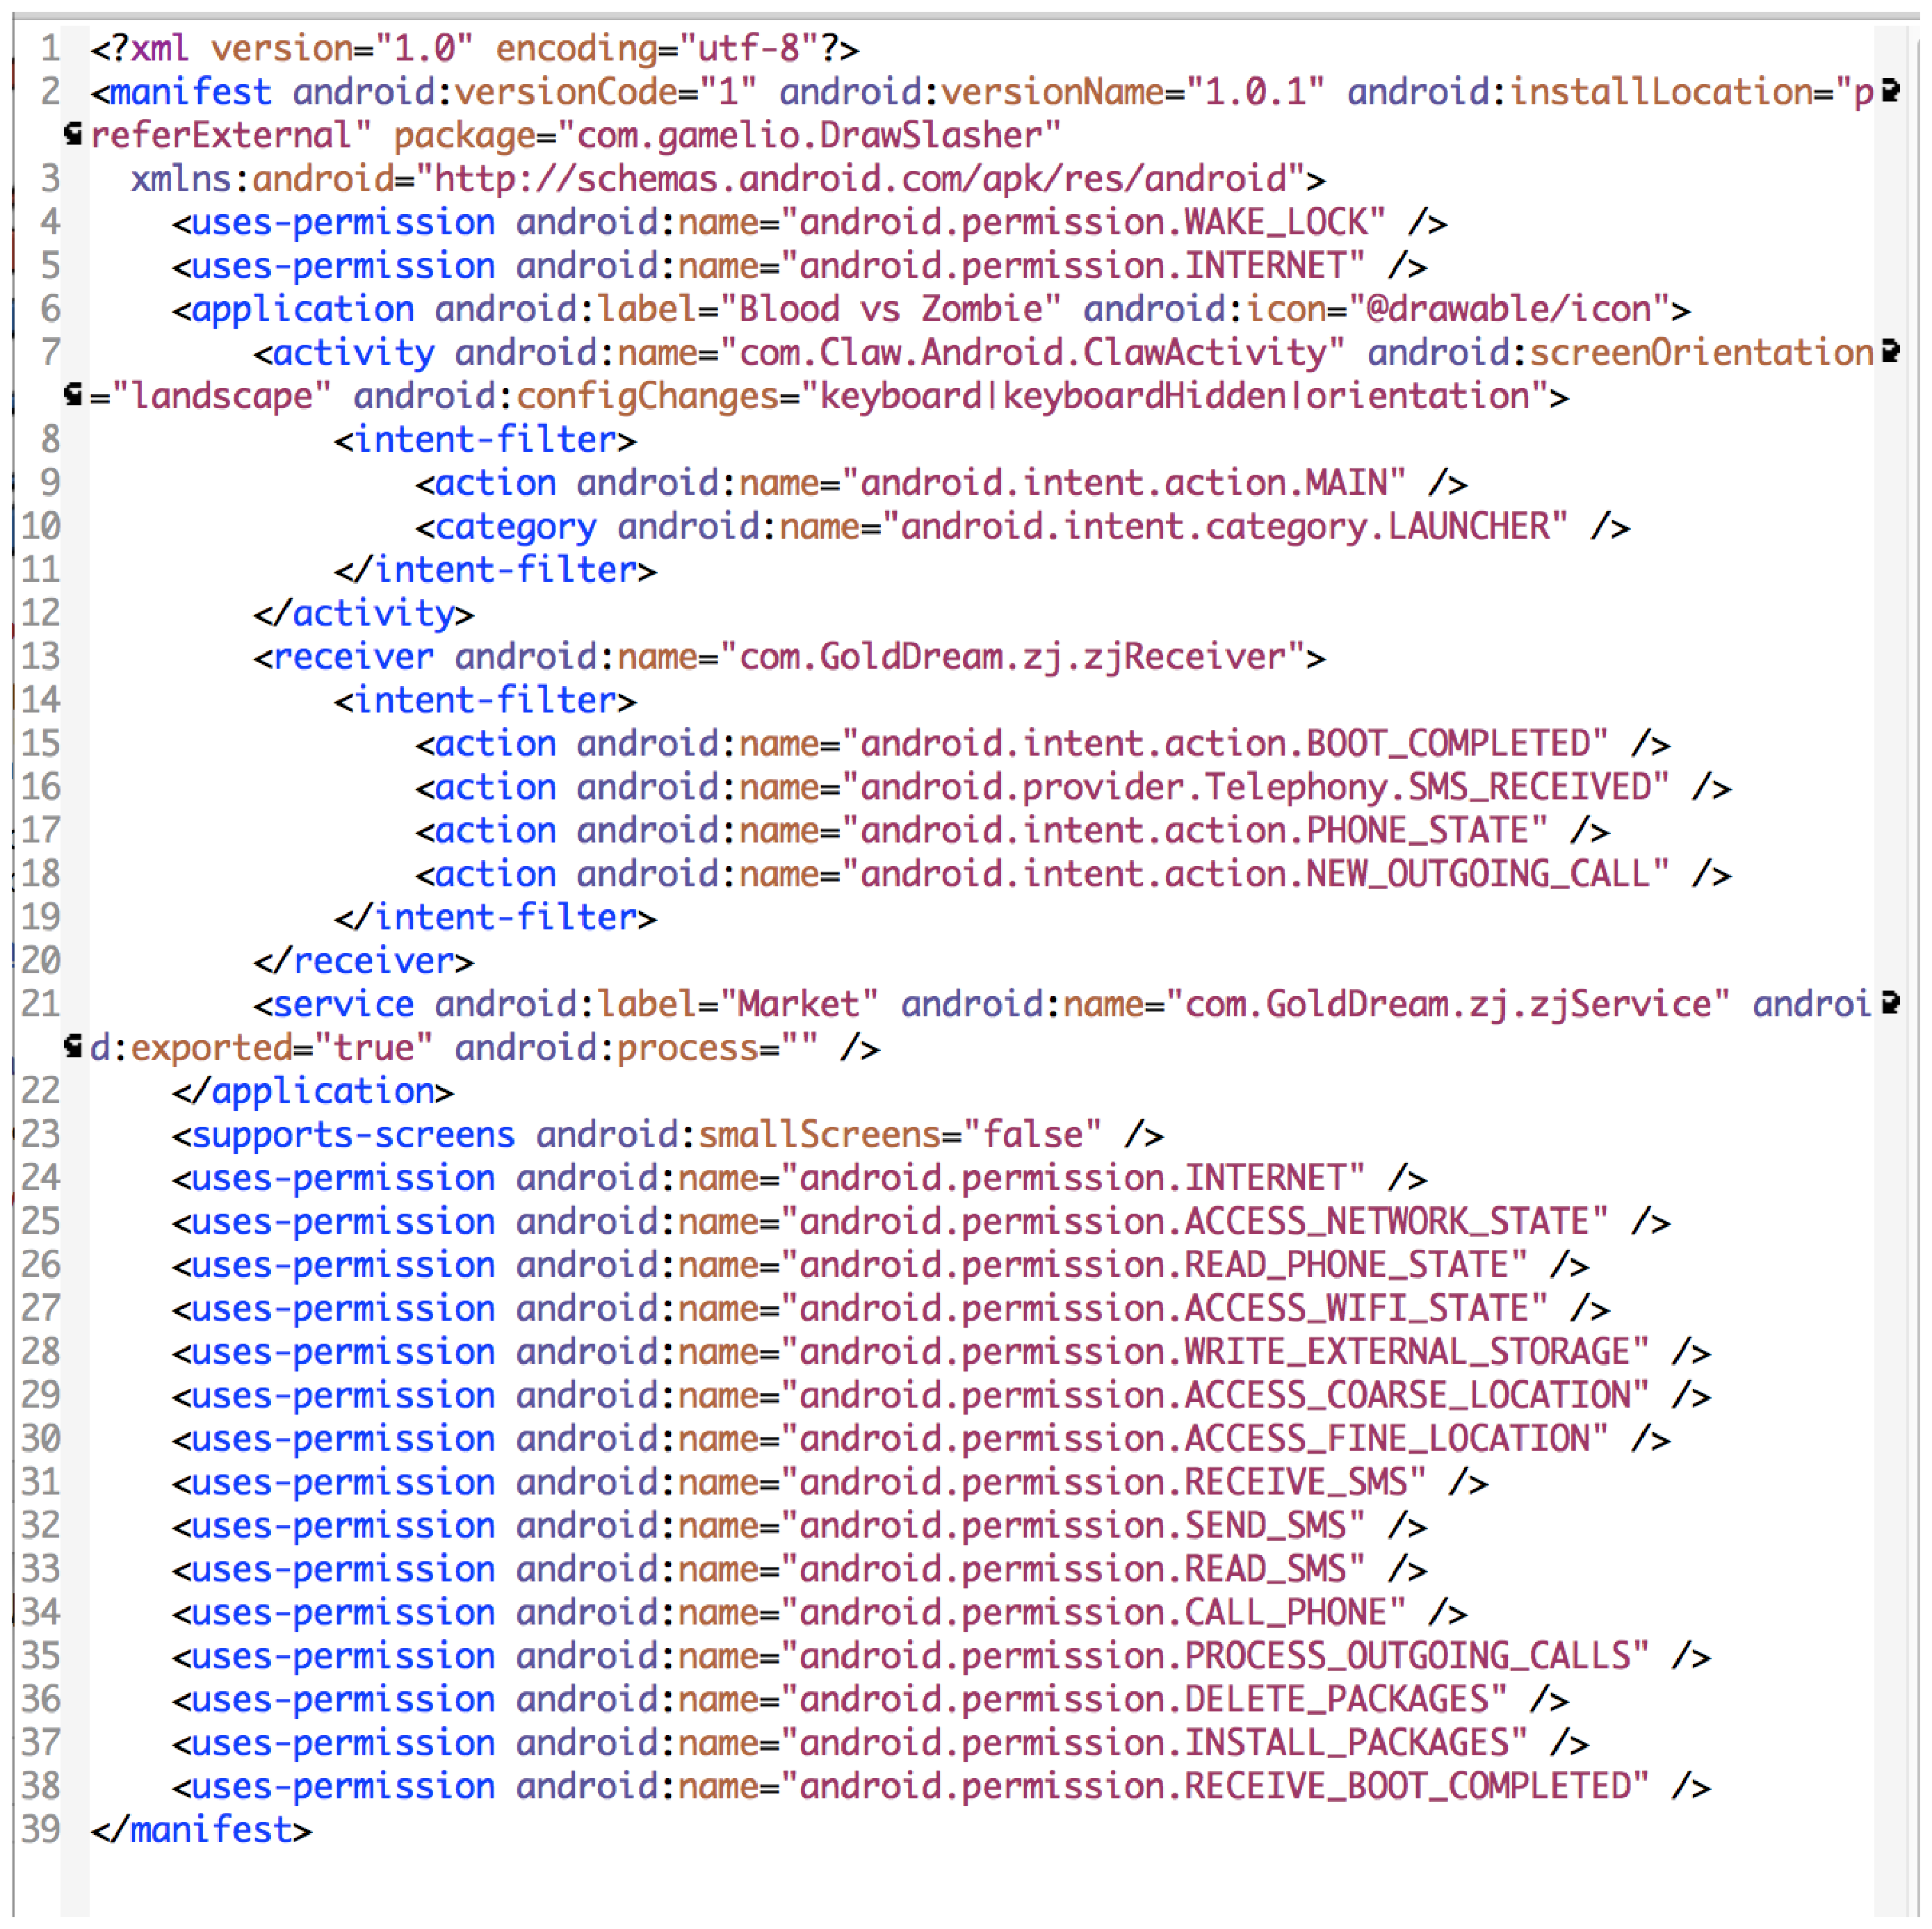
\includegraphics[ width= 125mm]{manifest2.eps}
\end{center}
\caption{AndroidManifest.xml の例}
\label{manif}
\end{figure}

classes.dex は,Android アプリの DEX コード実行ファイルである.DEX コードとは,Android 上で動く VM,Dalvik VM の中間言語だ.Android アプリの APK ファイル内には,必ず classes.dex は 1 つしか存在しないことになっている.二つ以上の .dex ファイル(例えば,classes.dex と classes1.dex)を APK ファイル内に入れることはできるが,実行するときは classes.dex のみが実行される.アプリのソースコードの全てのクラスファイルの中身が 1 つの DEX コードに変換される.Java VM も中間言語である,Java バイトコードを用いている.Javaでは,コンパイル時にクラス毎に Java バイトコードのファイル,クラスファイルが生成される.しかし,Dalvik VM では,アプリごとに DEX コードのファイル (classes.dex) が生成される.Android アプリを実装していた場合,自分が書いた Java ファイル (.java) がコンパイルされて Java クラスファイル (.class) に変換され,そのクラスファイルが 1 つの DEX コードファイルにまとめられるという流れになる.つまり, Java で実装されたソースコード中のクラスとは関係なく,1 つのファイルになる.また,dex2jar \cite{d2jar} というツールにより,classes.dex を JAR 形式に変換することができる.JAR ファイルは Java バイトコードが圧縮されたファイルであるから,これを解凍することで,Android アプリのクラスファイルを手に入れることができる.また,Android SDK が提供する dx というコマンドラインツールを用いることで,jar ファイルから DEX コードファイルを作成することもできる.本提案ではこれらの方法を用いてマルウェアのクラスファイルを入手し,そこから  classes.dex を作成した.

\newpage
\section{関連研究}
 Android マルウェアを解析,調査した研究を 3 つ紹介する.

Y.Zhou, X.Jiang は,2010 年の 8 月から 2011 年の10 月にかけて,公式サイト,非公式サイトから収集した 1,260 個,49 種類のAndroid マルウェアを用いて時系列調査と分類調査を行っている.時系列調査では,この研究で収集しているマルウェアの数 (dataset) をグラフで示している.DroidKungFu が登場した 2011 年 6 月,AnserverBot が登場した 2011 年 10 月にこの dataset の数が急激に増えた.つまり,この 2 つのマルウェアが大きな影響を及ぼしていることがわかる.分類調査では,マルウェアのインストールの方法,起動トリガー,挙動,マルウェアが要求する権限を調査している.49 種類中,25 種類のマルウェアが Repackage によりインストールされていた.マルウェアの起動トリガーとして最も多かったのは,OS の起動時で,29 種類だった.マルウェアの挙動は,Financial charge が最も多く,その中でも,SMS を使っているものが多かった.また,多くのマルウェアが SMS, Wi-Fi に関する権限を要求していた.また,先に出てきた,2 つのマルウェアがどのような挙動をするかを示している.DroidKungFu は6 種類のヴァージョンが見つかっており,外部サーバのアドレスの格納方法がジョジョジョに複雑になっている.AnserverBot は解析回避と遠隔操作の2 つの特徴を持つ.さらに,既存の 4つのセキュリティソフトがこの  dataset を検知するかどうかの調査も行った.その結果,最高は Lookout の 79.6 \% , 最低は Norton の 20.2 \% で,どのソフトウェアも検知できないマルウェアも存在した.この結果より,この 4 つのセキュリティソフトはまだ不十分であることがわかる.これらの調査結果からこの研究の結論として,マルウェアのインストール方法の中でも,最も頻繁に行われている Repackage を検知することとアプリの外部のコードの動的ローディングを防ぐ技術が必要であると彼らは主張している.この研究は Android マルウェアを調査,分類し,さらに 2 つのマルウェアについて詳しく挙動を示している.この研究では,解析手段(静的か動的か)までは言及していない.本研究では調査,分類は行わず,解析のみを行っている.

S.Poeplau らは,マルウェアの動的に外部コードの動的ローディングに焦点をおいて解析を行っている.\ref{sec:malware} で述べたように,外部コードのローディングをすることで公式ストアの検知システムをくぐり抜けることができる.また,外部コードのローディングは必ずしも不正なものではなく,マルウェア以外のアプリでも使われている.しかし,Android OS はロードされたコードをチェックしないので攻撃者はロードするものを置き換えることができる.そのためこれは Android アプリの脆弱性といえる.そこで,この研究で彼らは外部コードの動的ローディングを検知するツールを提案している.このツールは APK ファイルから取り出した DEX コードを静的に解析する.100 万回以上インストールされた,1,632 個のアプリをランダムに選び,このツールを用いて検査した.その結果,その中の 9.25 \% から外部コードのローディングの脆弱性が検知された.さらに,Google Play  での人気 50 位以内の無料アプリを同じツールで検査すると,16 \% ものアプリがその脆弱性を示した.また,彼らはこの攻撃手法に対する防御策も提案している.Dalvik VM が外部からダウンロードされたコードのハッシュ値を計算し,それが Whitelist に載っていなければ,それを実行できないようにアプリケーションに制限をかける.そうすることで,これを利用した攻撃を防ぐことができる.この研究での外部コードのローディングを検知するツールは,静的に行っているため,マルウェアを全く動かしていない.それに対して本研究ではマルウェアを実機で実際に動かして動的にログを得ることで解析している.また,この研究では,ひとつの攻撃手法に限定して解析を行っているが,本研究では,特定の攻撃手法に限定していない.

L.Yan, H.Yin はマルウェアの動的解析環境 (DroidScope) を提案している.彼らは Android SDK が提供するエミュレータをベースに自分たちで手を加えて,そのエミュレータの中でマルウェアを動かしている.彼らは Android システム全体の再構築を行っている.つまり,DroidScope はハードウェア,Linux OS (Android は Linux をベースにして動作している),Dalvik VM の 3 種類の API を提供する.DroidScope が提供する API を用いることで,Android API, Dalvik VM, Linux , さらには機械語の命令までをトレースするツールを提案している.{\it API tracer, native tracer, Dalvik instruction tracer} の 3 つである.また,これらの API に動的な taint analysis を実行することで,情報漏えいを解析するツール ({\it Taint tracker}) も提案している.彼らはこの 4 つのツールのパフォーマンス測定も行っている.元のエミュレータで実行時間を基準に,4 つのツールの実行時間を調べた.その結果,オーバーヘッドは小さいと言える結果であった.しかし,taint traker は他の 3 つのツールとくらべて大きなオーバーヘッドを示した.彼らはこれらのツールを用いて先に述べた,DroidKungFu を解析した.この解析によって,このマルウェアのルート権限を取得する方法と情報を盗み出す方法を明らかにしている.DroidKungFu だけでなく,論文中では DroidDream も解析している.DroidKungFu の場合と同様な解析を行った結果,DroidDream が端末識別番号を盗み出す方法を突き止めた.彼らの研究は実行された API,メソッドを動的に得ることで解析を行っているため,解析のためのアプローチは本研究と共通している点がある.しかし,本研究は実機で行っているのに対して,彼らの研究はエミュレータ上で行っている.もし,マルウェアがエミュレータ上で動作しているのを検知して,振る舞いを変える可能性もある.そのため,実機で解析すればマルウェアの "正常" な動作を解析することができる.

ここで紹介した研究には問題点が残っている.外部コードの動的ローディングの応用例として,文字列としてクラス名,メソッド名を受け取り,  reflection を通して実行することが考えられる.S.Poelau らの研究では外部コードの動的ローディングの攻撃を防ぐツールを提案したが,reflection を使うと,このツールでは検知することができない.DroidScope は動的解析のため,コードカバレッジが制限される.実行時には,1 つの実行パスしか通ることはない.L.Yan, H.Yin は実行パスを増やすために,システムコール,ネイティブ API,Dalvik メソッドなどの返り値を変えることで,異なる実行パスを実現した.symbolic execution のほうが,より良いことが考えられるが,かれらはこれを今後の課題としている.
(Crowdroid: behavior-based malware detection system for android ?)

\newpage
\section{提案}
本研究では,Android を標的にしたマルウェアの動的解析を行う.マルウェアにログコードを挿入させ,そのログを動的に得ることで解析を行う.エミュレータでは再現できないために解析できないことも,本提案では,実機でマルウェアを動かすため解析できるメリットがある.\ref{overview} では,本提案の全体の流れを説明する.\ref{placeinsert} では,ログコードをどのように挿入するかについて説明する.
\subsection{全体の流れ}
\label{overview}

\subsection{ログコードの挿入箇所}
\label{placeinsert}
\subsubsection{メソッドの先頭にコードを挿入}
 
\subsubsection{メソッド呼び出しの前後でコードを挿入}

\newpage
\section{実験}
\label{sec:exp}
じっけん
\subsection{目的}

\subsection{実験方法}

\subsection{実験結果}


\newpage
\section{おわりに}
\label{sec:concl}
おわりに
\subsection{まとめ}

\subsection{今後の課題}

\newpage
\section*{謝辞}
\addcontentsline{toc}{section}{謝辞}
\addcontentsline{toc}{section}{参考文献}
\begin{thebibliography}{9}
	\bibitem{osshare} IDC Smartphone OS Market Share, Q3 2014 \\http://www.idc.com/prodserv/smartphone-os-market-share.jsp
	\bibitem{cisco} Cisco 2014 Annual Security Report
	\bibitem{dissect} Yajin Zhou Xuxian jiang "Dissecting Android Malware: Characterization and Evolution" In {\it IEEE Symposium on Security and Privacy}, pages 95 - 109, 2012.
	\bibitem{aguard} androguard https://code.google.com/p/androguard/
	\bibitem{dbox} droidbox https://code.google.com/p/droidbox/
	\bibitem{d2jar} dex2jar https://code.google.com/p/dex2jar/
	\bibitem{sopho} SOPHOS Security Threat Report 2014
	\bibitem{remote ctrl} TrendLabs Security Intelligence Blog\\http://blog.trendmicro.com/trendlabs-security-intelligence/android-malware-found-to-send-remote-commands/
	\bibitem{droiddream} Security Alert: New Android Malware -- {\it GoldDream} -- \\http://www.cs.ncsu.edu/faculty/jiang/GoldDream/
	\bibitem {droidscope} 
	\bibitem{dynamicload} 
	
\end{thebibliography}
\end{document}